%%%%%%%%%%%%%%%%%%%%%%%%%%%%%%%%%%%%%%%%%%%%%%%%%%%%%%%%%%%%%%%%%%%%%%%%%%%%%%%%
\section{Spacecraft Tracking \& Observation Models}
%%%%%%%%%%%%%%%%%%%%%%%%%%%%%%%%%%%%%%%%%%%%%%%%%%%%%%%%%%%%%%%%%%%%%%%%%%%%%%%%

It should be noted that significant work towards the incorporation of laser
tracking for Lunar~\cite{Bauer2016, Bauer2017} and planetary science missions
have been carried out, and has demonstrated that range observations may be
improved by 2 orders of magnitude~\cite{Dirkx2019}. However, the primary purpose
of this research is the autonomous planning for the safe exploration of small
bodies, therefore the use of Interplanetary Laser Ranging (ILR) is considered
beyond the current scope, and is not covered by this work.

%In order to provide a fundamental view of estimation in the context of space
%missions, we generalize across what is implied by tracking, observation, and
%characterization of the space environment. Information is transmitted to an
%observer in the form of a signal, which has some identity associated to it.
%This signal is then

%%%%%%%%%%%%%%%%%%%%%%%%%%%%%%%%%%%%%%%%%%%%%%%%%%%%%%%%%%%%%%%%%%%%%%%%%%%%%%%%
\subsection{Radar Tracking}
%%%%%%%%%%%%%%%%%%%%%%%%%%%%%%%%%%%%%%%%%%%%%%%%%%%%%%%%%%%%%%%%%%%%%%%%%%%%%%%%

Radar tracking facilitates the determination of specific physical information of
a spacecraft, with respect to the path of signals taken though the defining
link-ends: transmitter and receiver, and in some configurations, transponders
(transmission of a signal in response to a received signal). The components of
physical information determinable between link-ends are:

\begin{enumerate}
    \item \textit{pointing angles}: determined by either (a) measuring the
    direction of the maximum signal amplitude of the spacecraft with respect to
    a single observer, or (b) Very Long Baseline Interferometry (VLBI) using
    multiple observers, given accurate relative fixed positions of the
    observers.
    \item \textit{range}: \textit{a.k.a. line-of-sight distance}, determined by
    the measuring the light trip time between A and B. This is most configured
    such that round-trip light time is measured, the duration between the
    emission of a signal from A, reflected at B, and received again by A.
    One-way configuration is also possible, with more stringent requirements on
    time precision.
    \item \textit{range rate}: \textit{a.k.a. line-of-sight velocity}, of
    a B with respect to an observer A can be derived from the Doppler shift
    of a radar wave. The most common configurations for these measurements are
    one-way, two-way and three-way.
\end{enumerate}

Radar tracking is the most used widely used form deep space spacecraft tracking
and is facilitated by a network of dedicated ground stations. Two popular
networks used in contemporary deep space spacecraft tracking are ESA's tracking
station network (ESTRACK) \cite{Doat2018} and NASA's Deep Space Network (DSN)
\cite{Dsn2015}. These networks generally operate in the X-band or Ka-band, or
both to account for dispersive propagation media \cite{Bertotti1993}. These
bands are designated by the International Telecommunication Union (ITU)
\cite{Berner2020}, and given in \autoref{tab:itu-bands}.

\begin{table}[htp!]
\renewcommand{\arraystretch}{1.5}
\centering
\caption{
    \textbf{Frequency Bands Allocated by the International Telecommunication
    Union (ITU)}. Near space bands are used for spacecrafts less than 2 million
    km from Earth, and deep space bands for any distance greater. *Deep Space
    S-band is not available at Madrid tracking stations due to a conflict with
    IMT- 2000 users, per agreement between NASA and Secretaria de Estado de
    Telecomunicaciones para la Sociedad de la Informacion (SETSI), January 2001
    ~\cite{Berner2020}.
}
\label{tab:itu-bands}
\begin{tabular}{lllll}
\hline
Band             & \multicolumn{2}{l}{Deep Space Bands} (MHz) & \multicolumn{2}{l}{Near Space Bands} (MHz)\\
                 &                                              Uplink & Downlink &                                             Uplink & Downlink  \\
\hline\hline
          S      &                                        2110–2120* &                    2290–2300 &                                        2025–2110 &                2200–2290 \\
          X      &                                        7145–7190  &                    8400–8450 &                                        7190–7235 &                8450–8500 \\
          K      &                                              N/A  &                          N/A &                                      22550-23150 &              25500–27000 \\
         Ka      &                                      34200–34700  &                  31800–32300 &                                              N/A &                       N/A \\
\hline
\end{tabular}
\end{table}

%%%%%%%%%%%%%%%%%%%%%%%%%%%%%%%%%%%%%%%%%%%%%%%%%%%%%%%%%%%%%%%%%%%%%%%%%%%%%%%%
\subsubsection{Deep Space Network (DSN)}
%%%%%%%%%%%%%%%%%%%%%%%%%%%%%%%%%%%%%%%%%%%%%%%%%%%%%%%%%%%%%%%%%%%%%%%%%%%%%%%%

The Deep Space Network (DSN) first developed the unified S-band (USB) system for
spacecrafts during the 1960s, during the Apollo missions~\cite{Peltzer1966}. It
has since been accompanied by the X-band, K-band and most recently, the Ka-band.
The network consists of three Deep Space Communication Complexes (DSCCs) located
in Goldstone California (GDSCC), Canberra Australia (CDSCC), and Madrid Spain
(MDSCC) with varying antenna sizes and types~\cite{Pham2020}. The frequency band
allocations designated by the International Telecommunication Union (ITU), as
used by the DSN, are provided in \autoref{tab:itu-bands}. There are three common
data types observed with the DSN \cite{Berner2020}:

\begin{itemize}
    \item \textit{One-way}: The spacecraft generates the downlink signal(s) from an
    onboard oscillator. The DSN compares the received frequency against a
    locally generated frequency
    \item \textit{Two-way}: The DSN transmits a signal to the spacecraft. The spacecraft
    tracks the phase of the uplink signal and generates a phase coherent
    downlink signal. The DSN compares the received frequency with the same
    reference frequency from which the uplink was generated.
    \item \textit{Three-way}: The spacecraft is tracked by two stations, one with the
    two-way mode while the other receives and compares the signal to a locally
    generated frequency. The most common application of this mode is during the
    handover between stations at two different DSCCs.
    \item \textit{Coherent Three-way}: Coherent three-way tracking is three-way tracking
    when the transmitting and receiving stations share a common frequency
    reference. This is possible at all three DSCCs as all antennas at a
    complex share the same frequency reference.
\end{itemize}

\begin{figure}[H]
    \centering
    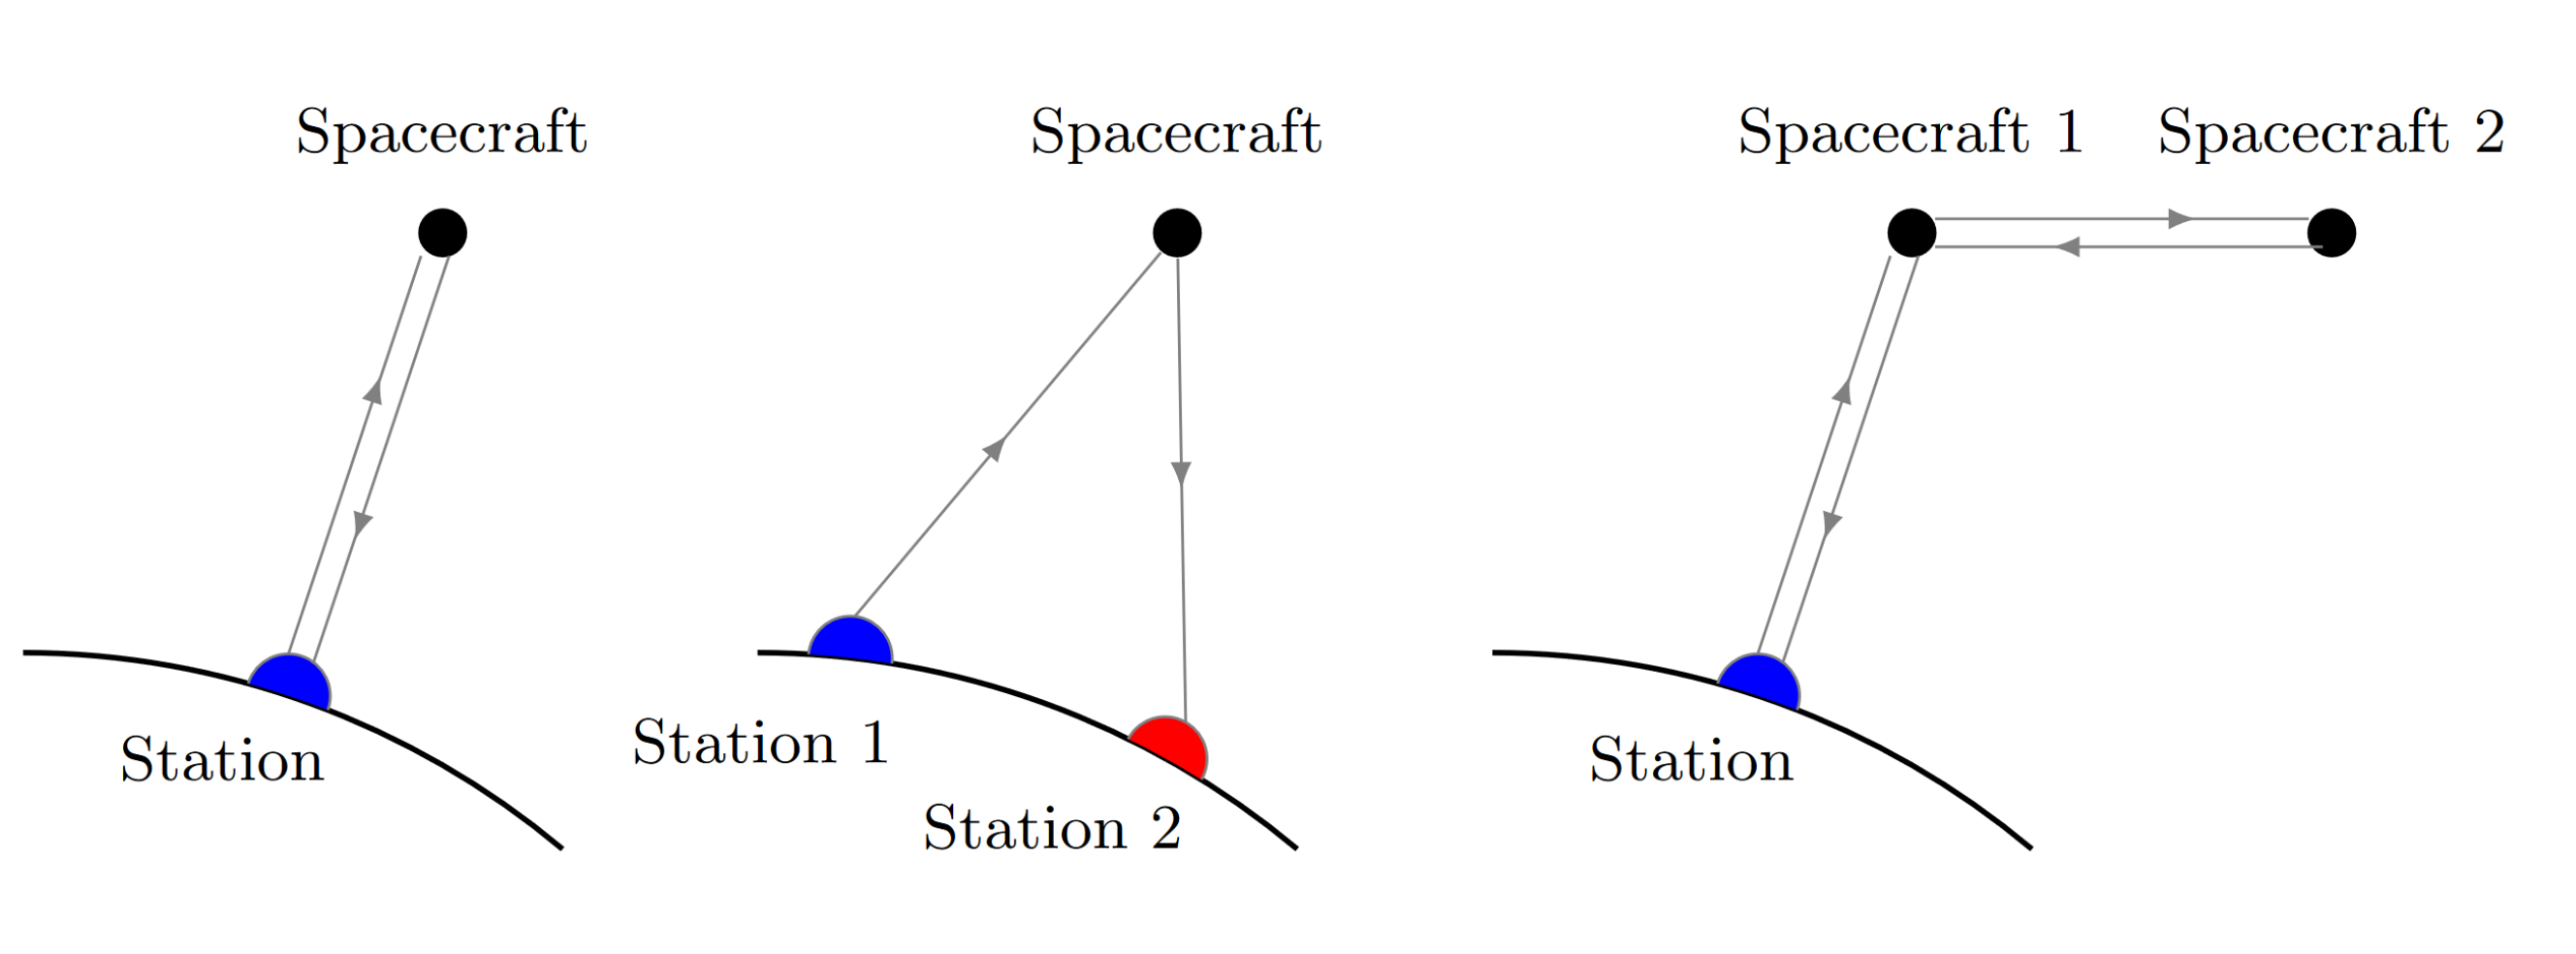
\includegraphics[width=0.85\linewidth]{graphics/n-way.PNG}
    \caption{
        \textbf{Schematic of \textit{n}-way observable data types} that are
        commonly facilltiated by the Deep Space Network (DSN). Depicted types
        are (left) two-way, (middle) three-way and (right) four-way. One-way is
        omitted, as it is simply the downlink of a spacecrafts signal to the
        ground station. This figure is taken from Dirkx \cite{Dirkx2015}.
    }
    \label{fig:n-way}
\end{figure}



%%%%%%%%%%%%%%%%%%%%%%%%%%%%%%%%%%%%%%%%%%%%%%%%%%%%%%%%%%%%%%%%%%%%%%%%%%%%%%%%
\subsubsection{Angle measurements}
%%%%%%%%%%%%%%%%%%%%%%%%%%%%%%%%%%%%%%%%%%%%%%%%%%%%%%%%%%%%%%%%%%%%%%%%%%%%%%%%

There are two primary methods of obtaining angle measurements of a spacecraft
relative to a ground station. The \textit{monopulse technique} obtains
antenna-angle offsets (a.k.a. boresight deviation) using two signals from the
spacecraft beacon: the difference signal $\Delta$ and the sum signal $\sum$.
Depending on the distance between the monopulse antenna and the spacecraft, and
the frequency of the signal, accuracies can range between 0.05 and 0.2 mrad
~\cite[p.~196]{Montenbruck2000}.

\begin{equation}
    \tau_g=\frac{1}{c}\bm{B}\cdot{\hat{\bm{s}}}.
    \label{eq:vlbi-vector}
\end{equation}

\begin{figure}
\centering
\begin{subfigure}{.48\textwidth}
  \centering
  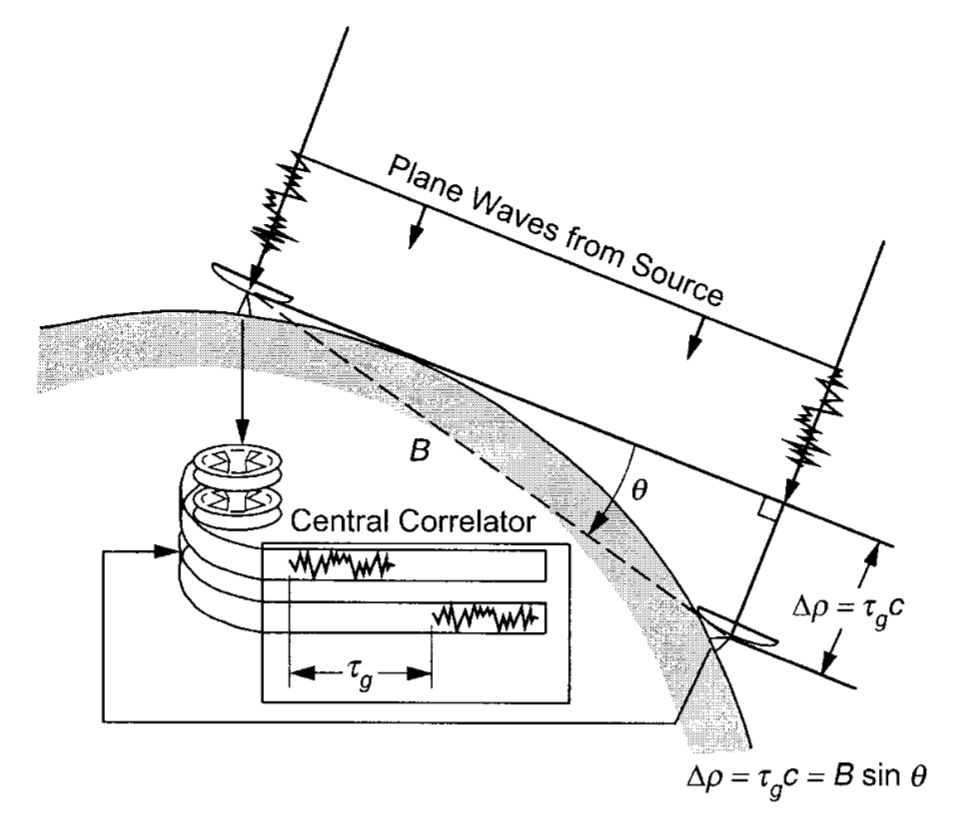
\includegraphics[width=.99\linewidth]{graphics/vlbi.PNG}
  \caption{
      \textbf{Measuring angles with VLBI}. Differential signal arrival time,
      $\tau_g$, is obtained by cross-correlating signals recorded open loop at
      each end of the baseline~\cite[p.~48]{Catherine2005}.
  }
  \label{fig:monopulse}
\end{subfigure}\hspace{0.03\textwidth}
\begin{subfigure}{.48\textwidth}
  \centering
  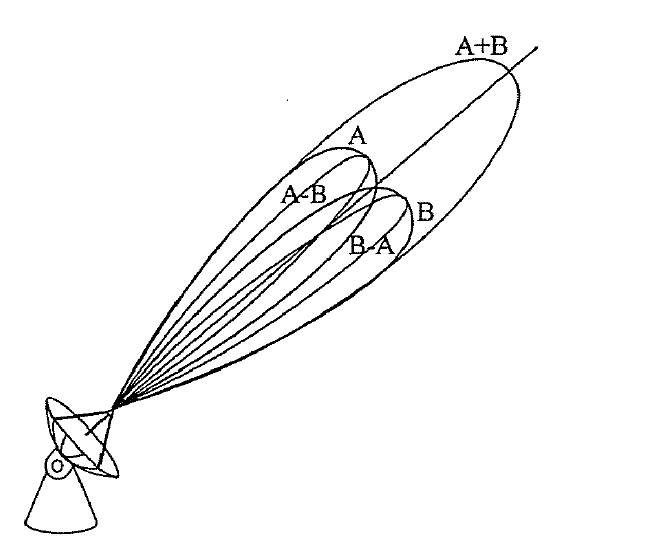
\includegraphics[width=.99\linewidth]{graphics/monopulse.PNG}
  \caption{
      \textbf{Measuring angles with the monopulse technique}. Antenna beams of a
      monopulse autotrack system.~\cite[p.~196]{Montenbruck2000}
  }
  \label{fig:vlbi}
\end{subfigure}
\caption{

}
\label{fig:test}
\end{figure}


%%%%%%%%%%%%%%%%%%%%%%%%%%%%%%%%%%%%%%%%%%%%%%%%%%%%%%%%%%%%%%%%%%%%%%%%%%%%%%%%
\subsubsection{Round-trip light time (RTLT) measurements}
%%%%%%%%%%%%%%%%%%%%%%%%%%%%%%%%%%%%%%%%%%%%%%%%%%%%%%%%%%%%%%%%%%%%%%%%%%%%%%%%

The most common radar ranging technique involves two-way ranging, the
transmission of a signal from A to B, and back to A, from which the signal
travel time $\tau$ is determined (as seen in \autoref{fig:n-way}). This is
expressed as the range value $\rho=1/2\cdot{}c\tau$ which is a measure of the
average of the uplink and downlink distance, as apposed to an instantanenous
measure. The variance of the range measurement can be expressed in meters, or in
seconds, where their relationship is expressed as \cite{Berner2002}:

\begin{equation}
    \sigma_{\rho}^2 = c^2\sigma_{\tau}^2
\end{equation}

The phase shift $\Delta\Phi$ is directly proportional to the
turn-around signal travel time through:

\begin{equation}
    \tau = \frac{\Delta\Phi}{2\pi{}f_0}
\end{equation}
%\begin{equation*}
%    \begin{aligned}
%    \text{where  }
%        f_0 &= \text{carrier signal frequency, }
%    \end{aligned}
%\end{equation*}

where $f_0$ is the carrier signal frequency. There are two main systems used in
RTLT ranging, namely \textit{tone-ranging systems} and \textit{code ranging
systems}, as depicted in \autoref{fig:ranging-methods}. Both systems have their
own advantages and disadvantages. Tone-ranging measurements suffer from
ambiguity which can be mitigated through the use of additional sub-harmonic
tones, whereas code-ranging requires greater acquisition time for weak signals,
unless a pre-steering Doppler shift is used \cite[p.~197]{Montenbruck2000}.

\begin{figure}
    \centering
    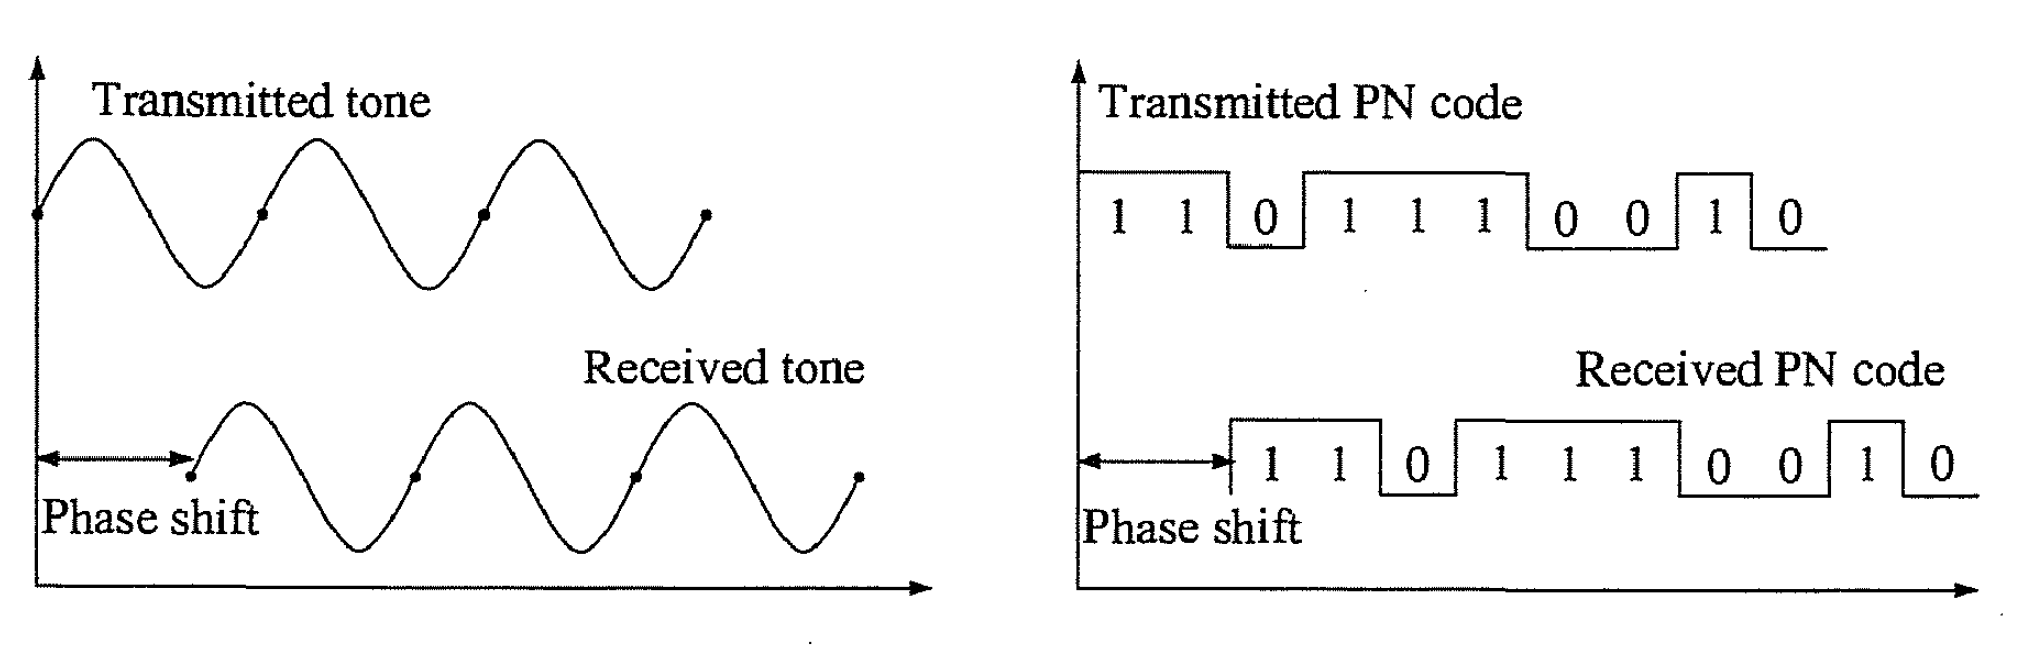
\includegraphics[width=1.0\linewidth]{graphics/ranging-method.PNG}
    \caption{
        \textbf{Primary physical principles behind Round-trip Light time (RTLT)
        ranging.}, shown are tone ranging (left) and code ranging (right)
        \cite[p.~196]{Montenbruck2000}
    }
    \label{fig:ranging-methods}
\end{figure}


%%%%%%%%%%%%%%%%%%%%%%%%%%%%%%%%%%%%%%%%%%%%%%%%%%%%%%%%%%%%%%%%%%%%%%%%%%%%%%%%
\subsubsection{Doppler measurements}
%%%%%%%%%%%%%%%%%%%%%%%%%%%%%%%%%%%%%%%%%%%%%%%%%%%%%%%%%%%%%%%%%%%%%%%%%%%%%%%%

To measure two-way or three-way Doppler shift, the spacecraft must transmit a
downlink signal that is phase coherent with the uplink signal.
\autoref{tab:turnaround-ratios} provides the recommended spacecraft transponder
turnaround ratios for various uplink and downlink frequency bands.

Doppler measurements are typically integrated of a period of about 60 seconds
\cite{}, however periods in the lower range of 1-10 seconds \cite{}, or larger
periods such as 1000 seconds may also be chosen \cite{}.


\cite{Soffel1989}

\begin{equation}
    \frac{f_r}{f_t} = \frac{
        1-\mathbf{v}_r\cdot{}\mathbf{e}/c + U_r/c^2 +\mathbf{v}_r^2/(2c^2)
    }{
        1-\mathbf{v}_t\cdot{}\mathbf{e}/c + U_t/c^2 +\mathbf{v}_t^2/(2c^2)
    }
\end{equation}
\begin{equation*}
    \begin{aligned}
        \textrm{where  }
        \mathbf{f}_t, \mathbf{f}_r &= \textrm{the transmitted and received signal frequencies,}\\
        \mathbf{v}_t, \mathbf{v}_t &= \textrm{the transmitters and receivers inertial velocity vectors,}\\
        \mathbf{e} &= \textrm{the unit vector in the direction of the signal propagation,}\\
        c &= \textrm{the speed of light,}\\
        \mathbf{U}_t, \mathbf{U}_r &= \textrm{the Newtonian potential at the trasmitter and receiver.}\\
    \end{aligned}
\end{equation*}

The frequency shift, $f_r/f_t$ cannot be measured instantaneously and must be
time averaged over a counting period, $t_c$


\begin{table}[htp!]
\renewcommand{\arraystretch}{1.5}
\centering
\caption{
    \textbf{Spacecraft Transponder Turnaround Ratios.} *K-band uplink
    implementation, at two 34-meter BWG antennas per complex, will start
    November 2021 and complete July 2024. **K-band Doppler and ranging data are
    not supported by the DSN. ***Due to the bandwidth difference between 600 MHz
    uplink and 1500 MHz downlink, the coherency between uplink and downlink
    using these transponder ratios does not apply to the entire allocated
    bandwidth~\cite{Berner2020}.
}
\label{tab:turnaround-ratios}
\begin{tabular}{lll}
\hline
\textbf{Uplink} & \textbf{Downlink} & \textbf{Ratio (downlink/uplink)}  \\
\hline\hline
S               & S                 & 240/221                           \\
S               & X                 & 880/221                           \\
S               & Ka                & 3328/221, 3344/221, 3360/221      \\
X               & S                 & 240/749                           \\
X               & X                 & 880/749                           \\
X               & $K_a$             & 3328/749, 3344/749, 3360/749      \\
K*              & K**               & 2407/2720, 2407/2760, 2407/2816***\\
$K_a$           & $K_a$             & 3344/3599, 3360/3599              \\
\hline
\end{tabular}
\end{table}

%%%%%%%%%%%%%%%%%%%%%%%%%%%%%%%%%%%%%%%%%%%%%%%%%%%%%%%%%%%%%%%%%%%%%%%%%%%%%%%%
\subsubsection{Two-way Doppler Measurements}
%%%%%%%%%%%%%%%%%%%%%%%%%%%%%%%%%%%%%%%%%%%%%%%%%%%%%%%%%%%%%%%%%%%%%%%%%%%%%%%%

\begin{equation}
    N = \int_{t_1}^{t_2}(f_r-f_{ref})dt
\end{equation}
\begin{equation*}
    \begin{aligned}
        \textrm{where  }
        \mathbf{f}_t, \mathbf{f}_r &= \textrm{the transmitted and received signal frequencies,}\\
        \mathbf{v}_t, \mathbf{v}_t &= \textrm{the transmitters and receivers inertial velocity vectors,}\\
        \mathbf{e} &= \textrm{the unit vector in the direction of the signal propagation,}\\
        c &= \textrm{the speed of light,}\\
        \mathbf{U}_t, \mathbf{U}_r &= \textrm{the Newtonian potential at the trasmitter and receiver.}\\
    \end{aligned}
\end{equation*}

\begin{equation}
    N = \int_{t_1}^{t_2}(f_r)dt-f_{ref}(t_2-t_1)
\end{equation}

\begin{equation}
    N = \int_{t_1}^{t_2}(f_r)dt = T_{1,2}\int_{t_1-\tau_1}^{t_2-\tau_2}
\end{equation}

\begin{equation}
    \dot{\rho} = \int_{t_1}^{t_2}(f_r)dt = T_{1,2}\int_{t_1-\tau_1}^{t_2-\tau_2}
\end{equation}

%%%%%%%%%%%%%%%%%%%%%%%%%%%%%%%%%%%%%%%%%%%%%%%%%%%%%%%%%%%%%%%%%%%%%%%%%%%%%%%%
%\subsubsection{Angle Measurements}
%%%%%%%%%%%%%%%%%%%%%%%%%%%%%%%%%%%%%%%%%%%%%%%%%%%%%%%%%%%%%%%%%%%%%%%%%%%%%%%%


%\subsubsection{Ranging}

%\subsubsection{Doppler Tracking}

%$t_c = t_2 - t_1$

%\subsection{Doppler Measurements}


%\subsubsection{Rational Doppler Bias}
%\textcolor{red}{No real need to discuss, cut out in post processing.}
%\begin{equation}
%    \delta\overline{\dot{\rho}} = \frac{1}{t_c}\int_{t-t_c}^{t}d\cdot{\omega\sin{\alpha}\sin{\omega{t}}\;dt}
%\end{equation}

%\begin{equation}
%    \Delta{\overline{\dot{\rho}}} = \frac{\lambda\omega}{2\pi}\frac{s_R+s_T/T_{1,2}}{2}
%\end{equation}



\subsection{Landmark Tracking}

Landmark tracking is facilitated by a perspective projection model, usually a
pin-hole camera model~\cite{Shuang2008} which allows for the mapping of 3D
positions to 2D image points, for simulation and navigational purposes.
Positions in the camera-fixed frame $(x^c, y^c, z^c)$, are mapped to pixel
points on the image plane $(u,v)$ according to the relations:

\begin{equation}
    \begin{aligned}
        u&=f\frac{x^c}{z^c},\\
        v&=f\frac{y^c}{z^c}.
    \end{aligned}
\end{equation}

The line-of-sight vector $b_i^c$ of the $i^{th}$ image point to the camera
exposure center in the camera-fixed frame is defined by:

\begin{equation}
    \mathbf{b}_i^c=\frac{1}{\sqrt{(\bar{x}_i^c)^2+(\bar{y}_i^c)^2+f^2}}
    \begin{bmatrix}
    -\bar{x}^c_i \\
    -\bar{y}^c_i \\
    -f \\
    \end{bmatrix},
\end{equation}

\begin{equation}
    \mathbf{I}_i^I=\frac{1}{\sqrt{(x^I_i - x^I)^2+(y^I_i - y^I)^2+(z^I_i - z^I)^2}}
    \begin{bmatrix}
    x^I_i - x^I \\
    y^I_i - y^I \\
    z^I_i - z^I \\
    \end{bmatrix},
\end{equation}

\begin{equation}
    \tilde{\mathbf{b}}_i^c=\mathbf{A}\mathbf{I}_i^I
\end{equation}


\begin{figure}[htp]
    \centering
    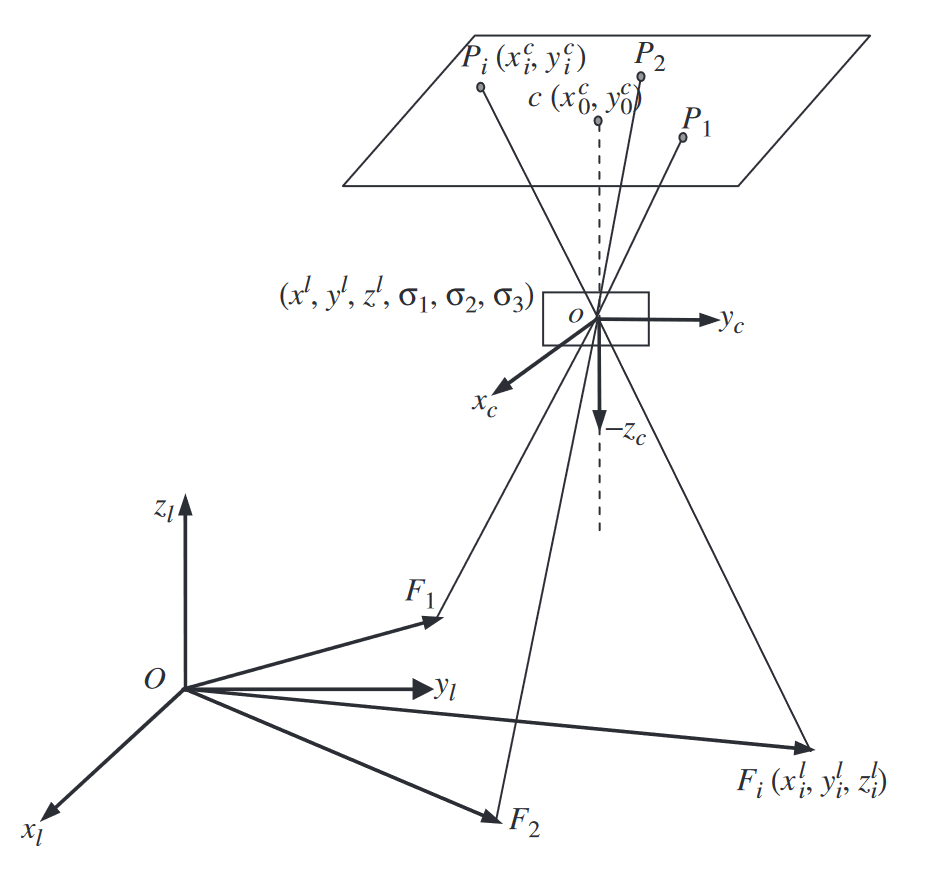
\includegraphics[width=0.55\linewidth]{graphics/landmark_geometry.PNG}
    \caption{
        \textbf{Relative geometrical relationship between spacecraft and landmarks
        for a pin-hole camera model}
    }
\end{figure}


%\textcolor{red}{Marie's Thesis + Michael. Model is similar to VLBI model.}
%
%\textcolor{red}{2.1.1 In D.Dirkx for better notation.}
%
%\textcolor{red}{Moyer, formulation for observed and computed quantities in DSN types.}

%%%%%%%%%%%%%%%%%%%%%%%%%%%%%%%%%%%%%%%%%%%%%%%%%%%%%%%%%%%%%%%%%%%%%%%%%%%%%%%%
\subsection{Tracking Data models}
%%%%%%%%%%%%%%%%%%%%%%%%%%%%%%%%%%%%%%%%%%%%%%%%%%%%%%%%%%%%%%%%%%%%%%%%%%%%%%%%

%%%%%%%%%%%%%%%%%%%%%%%%%%%%%%%%%%%%%%%%%%%%%%%%%%%%%%%%%%%%%%%%%%%%%%%%%%%%%%%%
\subsubsection{Light-time correction (aberration)}
%%%%%%%%%%%%%%%%%%%%%%%%%%%%%%%%%%%%%%%%%%%%%%%%%%%%%%%%%%%%%%%%%%%%%%%%%%%%%%%%

\textbf{one-way correction}

\begin{equation}
    \begin{aligned}
        \tau_{\underline{A}B}^{(i+1)}(t_t) &= \frac{1}{c}|\bm{r}_B(t_t+\tau_{AB}^{(i)})-\bm{r}_A(t_t)|\text{, transmitter (A) clamped} \\
        \tau_{A\underline{B}}^{(i+1)}(t_r) &= \frac{1}{c}|\bm{r}_B(t_r)-\bm{r}_A(t_r-\tau_{AB}^{(i)})|\text{, receiver (B) clamped}
    \end{aligned}
\end{equation}

\textbf{two-way correction}

\begin{equation}
    \begin{aligned}
        \tau_{\underline{B}A}^{(i+1)} &= \frac{1}{c}|\bm{r}_B(t+\tau_{AB})-\bm{r}_A(t+\tau_{BA}^{(i)})|\text{, transponder (B) clamped} \\
        \tau_{A\underline{B}}^{(i+1)} &= \frac{1}{c}|\bm{r}_B(t)-\bm{r}_A(t-\tau_{AB}^{(i)})|\text{, receiver (A) clamped}
    \end{aligned}
\end{equation}

%%%%%%%%%%%%%%%%%%%%%%%%%%%%%%%%%%%%%%%%%%%%%%%%%%%%%%%%%%%%%%%%%%%%%%%%%%%%%%%%
\subsubsection{Range}
%%%%%%%%%%%%%%%%%%%%%%%%%%%%%%%%%%%%%%%%%%%%%%%%%%%%%%%%%%%%%%%%%%%%%%%%%%%%%%%%

\textbf{RTLT}
\begin{equation}
    \overline{\dot{\rho}}(t) = \frac{c}{2}\frac{(\tau_{2u}+\tau_{2d})-(\tau_{1u}+\tau_{2d})}{t_c} = \frac{1}{2}\frac{(\rho_{2u}+\rho_{2d})-(\rho_{1u} + \rho_{1d})}{t_c},
\end{equation}


%%%%%%%%%%%%%%%%%%%%%%%%%%%%%%%%%%%%%%%%%%%%%%%%%%%%%%%%%%%%%%%%%%%%%%%%%%%%%%%%
\subsubsection{Range Rate}
%%%%%%%%%%%%%%%%%%%%%%%%%%%%%%%%%%%%%%%%%%%%%%%%%%%%%%%%%%%%%%%%%%%%%%%%%%%%%%%%

\textbf{Two-way Range Rate}
\begin{equation}
    \overline{\dot{\rho}}(t) = \frac{c}{2}\frac{(\tau_{2u}+\tau_{2d})-(\tau_{1u}+\tau_{2d})}{t_c} = \frac{1}{2}\frac{(\rho_{2u}+\rho_{2d})-(\rho_{1u} + \rho_{1d})}{t_c},
\end{equation}

%\subsubsection{Range}

\textbf{One-Way Range Rate}
\begin{equation}
    \overline{\dot{\rho}} = c\frac{(\tau_2-\tau_1)}{t_c}=\frac{(\rho_2-\rho_1)}{t_c}
\end{equation}


%\subsection{Doppler Measurements}
%
%\subsubsection{Two-way Range Rate}
%\begin{equation}
%    \overline{\dot{\rho}}(t) = \frac{c}{2}\frac{(\tau_{2u}+\tau_{2d})-(\tau_{1u}+\tau_{2d})}{t_c} = \frac{1}{2}\frac{(\rho_{2u}+\rho_{2d})-(\rho_{1u} + \rho_{1d})}{t_c},
%\end{equation}
%
%\subsubsection{Range}
%
%\subsubsection{One-Way Range Rate}
%\begin{equation}
%    \overline{\dot{\rho}} = c\frac{(\tau_2-\tau_1)}{t_c}=\frac{(\rho_2-\rho_1)}{t_c}
%\end{equation}
%
%\subsubsection{Rational Doppler Bias}
%\textcolor{red}{No real need to discuss, cut out in post processing.}
%\begin{equation}
%    \delta\overline{\dot{\rho}} = \frac{1}{t_c}\int_{t-t_c}^{t}d\cdot{\omega\sin{\alpha}\sin{\omega{t}}\;dt}
%\end{equation}
%
%\begin{equation}
%    \Delta{\overline{\dot{\rho}}} = \frac{\lambda\omega}{2\pi}\frac{s_R+s_T/T_{1,2}}{2}
%\end{equation}
%
%
%\newpage{}
%
%\begin{equation}
%    \rho = ||\mathbf{r}_\Sun - \mathbf{R}_\Earth||
%\end{equation}
%
%
%\begin{equation}
%    \rho = ||\mathbf{r}_\Sun - \mathbf{R}_\Earth||
%\end{equation}
%
%\begin{itemize}
%    \item \textbf{Orbit Determination}
%    \item
%\end{itemize}
%
%\subsection{Rotational State}
%
%\subsection{Gravitational Potential}
%
%\subsection{Shape}
%
%\begin{itemize}
%    \item \textbf{Rotation Model}:
%\end{itemize}